\section{The Poisson Equation}

The Poisson equation with dirichlet boundary conditions is
\begin{equation}
    - \Delta u = f, u(0) = a, u(1) = b
\end{equation}

Let \( \hat{K} = [0, 1] \) serve as the reference element.
The Lagrange interpolant polynomials (shape functions)
on the nodes \( (0, 1/2, 1) \) is
then
\begin{align}
  \Psi_0(x) &= 2x^2 - 3x + 1\\
  \Psi_1(x) &= -4x^2 + 2x\\
  \Psi_2(x) &= 2x^2 - x
\end{align}

We partition the interval \( K = [0, 1] \) into \( M + 1 \) points.
Given a partition \( 0 = s_0 < s_1 < \dots < s_M = 1  \)
we define the elements \( K_k = [s_{k}, s_{k+1}] \).
Denote the size of element \( k \) by \( h_k := s_{k+1} - s_{k} \).

In order to construct a basis on \( X_h^2 \) we need three
nodes per element.
Hence, a partition of \( K \) into \( M + 1 \) points
results in \( M \) segments and \( 2M + 1 \) nodes.
Let \( x_i \) denote the \( i \)'th node.

In the following we use \( k \) to indicate the index
of a segment and \( \alpha \in \{  0, 1, 2  \} \) to indicate
the node on the segment. These indices are related by the
local to global map \( \theta \):

\begin{equation}
  i = \theta(k, \alpha) := 2k + \alpha    
\end{equation}

TODO: A figure here perhaps?

Define the following maps:
\begin{align}
  \Phi_k : \hat{K} &\longrightarrow  K \\
  \xi & \longmapsto \xi s_{k+1} + (1-\xi) s_{k} \\
  \Phi_k^{-1} : K &\longrightarrow  \hat{K} \\
  x & \longmapsto \frac{x - s_k}{s_{k+1} - s_k}
\end{align}

The \( i \)'th basis function is denoted by \( \varphi_i \)
and is defined as
\begin{equation}
  \varphi_i(x) = \varphi_{\theta(k, \alpha)} := \Psi_{\alpha}({{\Phi_k}^{-1}(x) })
\end{equation}

\subsection{Setting up the weak form}

TODO: her kan me sikkert anta at lesaren veit korleis det blir gjort
og berre presentere resultater.

\subsection{Stiffness matrix and Load vector}

TODO: samme her kanskje? kor mykje skal med?

The elemental stiffness matrix and load vector has entries

\begin{align}
  [A^{K_k}]_{ij} &= \frac{1}{h_k} \int_{0}^{1} \Psi_i'(\xi)\Psi_j'(\xi) \,\mathrm{d}\xi \\
  [F^{K_k}]_j &= h_k \int_{0}^{1} f\left(\Phi_k\left(\xi\right)\right) \Psi_j\left(\xi\right) \,\mathrm{d}\xi
\end{align}

The elemental stiffness matrix is

\begin{equation}
  A^{K_k} = \frac{1}{3h_k}
  \begin{bmatrix}
  7 & -8 & 1\\
  -8 & 16 & -8\\
  1 & -8 & 7\\
  \end{bmatrix}
\end{equation}

\subsection{Test problem}

We use the test solution \( u(x) = x(x-1)\sin(3\pi x) \).

\begin{equation}
  \text{TODO}
\end{equation}

\begin{figure}[!h]
  \centering
  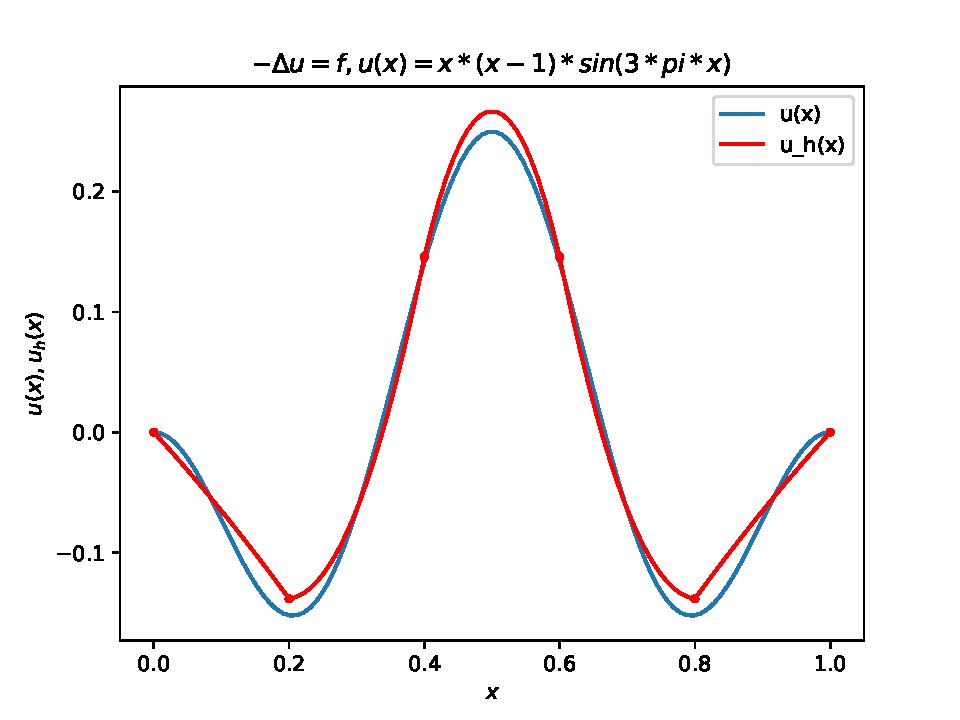
\includegraphics[width=0.75\textwidth]{Images/plots/task1_test_sol.pdf}
  \caption{TODO}
  \label{fig:test_eq}
\end{figure}

\subsection{Convergence analysis}


TODO: teoretisk utledning

\begin{theorem}
    Let $u \in H_0^3(\Omega)$ and $u_h \in X_h^2 \cap H_0^1$ be the solutions of the infinite and finite dimensional
    variational problem respectively, where $h$ is the maximum element size in $X_h^2$. Assume further that $F$ in the variational problem is bounded,
    and that $u$ has a second order polynomial interpolant $u_h^2$ on $\Omega$. Then
    \begin{equation}
        ||u - u_h||_{H^1} \leq Ch^2
    \end{equation}
    for some constant $C > 0$.
\end{theorem}
\begin{proof}
    We first note that $a(u, v)$ is both bounded and coercive. Combined with the assumption that $F$ is bounded, we then get from the Lax-Milgram \ref{}
    theorem that the variational problem admits a unique solution.
    
    From Cea's lemma \ref{} we then obtain
    \begin{equation}
        ||u - u_h||_{H^1} \leq \frac{M}{\alpha}||u - v_h||_{H^1} = \frac{M}{\alpha}(||u - v_h||_{L^2} + |u - v_h|_{H^1}) \quad \forall v_h \in X_h^2 \cap H_0^1.
    \end{equation}
    Since $u(0) = u(1) = 0$, and $\{0, 1\}$ are nodes of the interpolating polynomial, we obtain that $u_h^2(0) = u_h^2(1) = 0$ as well.
    In particular we get that $u_h^2 \in X_h^2 \cap H_0^1$.
    
    Choosing $v_h = u_h^2$ in Cea's lemma results in 
    \begin{equation}
        ||u - u_h||_{H^1} \leq \frac{M}{\alpha}(||u - u_h^2||_{L^2} + |u - u_h^2|_{H^1}),
    \end{equation}
    which combined with lemma 4.4 \ref{} gives us
    \begin{equation}
        \begin{aligned}
            \frac{M}{\alpha}||u - v_h||_{H^1} &\leq \frac{M}{\alpha}(C_{2}h^3|u|_{H^3} + C_{1}h^2|u|_{H^3}) \\
            &= h^2\frac{M}{\alpha}(C_{2}h|u|_{H^3} + C_{1}|u|_{H^3}) \\
            &= Ch^2
        \end{aligned}
    \end{equation}
\end{proof}


\subsubsection{Numerical Verification}


\begin{figure}[!h]
  \centering
  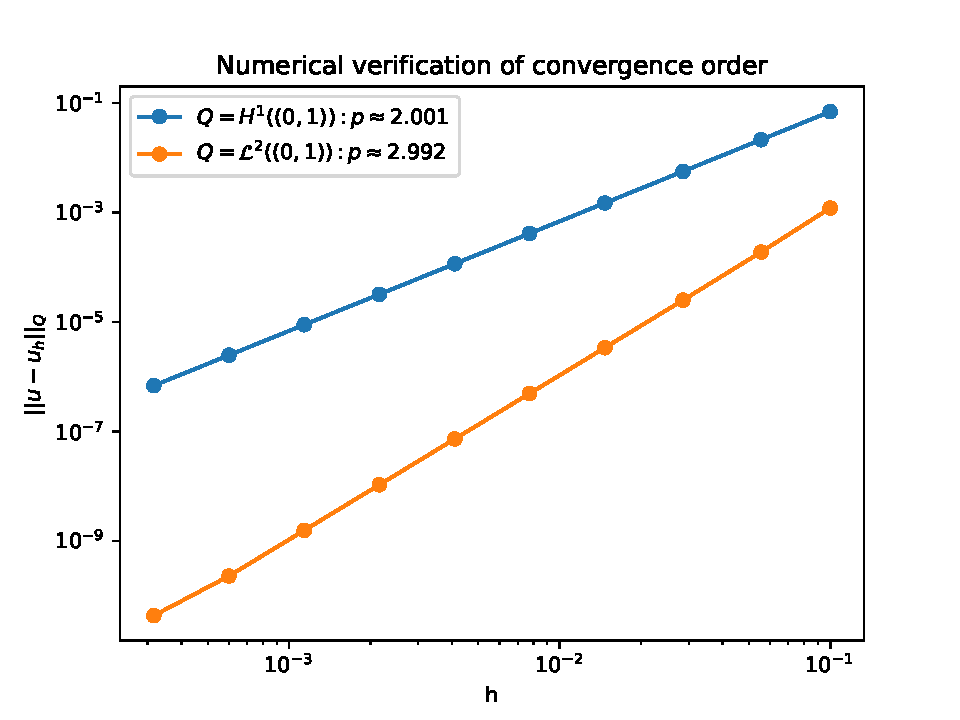
\includegraphics[width=0.75\textwidth]{Images/plots/task1_conv_plot.pdf}
  \caption{TODO}
  \label{fig:conv_plot}
\end{figure}

